\documentclass[journal]{IEEEtran}

\ifCLASSINFOpdf
  % \usepackage[pdftex]{graphicx}
  % declare the path(s) where your graphic files are
  % \graphicspath{{../pdf/}{../jpeg/}}
  % and their extensions so you won't have to specify these with
  % every instance of \includegraphics
  % \DeclareGraphicsExtensions{.pdf,.jpeg,.png}
\else
  % or other class option (dvipsone, dvipdf, if not using dvips). graphicx
  % will default to the driver specified in the system graphics.cfg if no
  % driver is specified.
  % \usepackage[dvips]{graphicx}
  % declare the path(s) where your graphic files are
  % \graphicspath{{../eps/}}
  % and their extensions so you won't have to specify these with
  % every instance of \includegraphics
  % \DeclareGraphicsExtensions{.eps}
\fi
% graphicx was written by David Carlisle and Sebastian Rahtz. It is
% required if you want graphics, photos, etc. graphicx.sty is already
% installed on most LaTeX systems. The latest version and documentation
% can be obtained at: 
% http://www.ctan.org/pkg/graphicx
% Another good source of documentation is "Using Imported Graphics in
% LaTeX2e" by Keith Reckdahl which can be found at:
% http://www.ctan.org/pkg/epslatex
%
% latex, and pdflatex in dvi mode, support graphics in encapsulated
% postscript (.eps) format. pdflatex in pdf mode supports graphics
% in .pdf, .jpeg, .png and .mps (metapost) formats. Users should ensure
% that all non-photo figures use a vector format (.eps, .pdf, .mps) and
% not a bitmapped formats (.jpeg, .png). The IEEE frowns on bitmapped formats
% which can result in "jaggedy"/blurry rendering of lines and letters as
% well as large increases in file sizes.
%
% You can find documentation about the pdfTeX application at:
% http://www.tug.org/applications/pdftex

% *** PDF, URL AND HYPERLINK PACKAGES ***
%
\usepackage{url}
% url.sty was written by Donald Arseneau. It provides better support for
% handling and breaking URLs. url.sty is already installed on most LaTeX
% systems. The latest version and documentation can be obtained at:
% http://www.ctan.org/pkg/url
% Basically, \url{my_url_here}.
\usepackage{amsmath,amssymb,amsfonts}
\usepackage{algorithm,algorithmic}
\usepackage{graphicx}
\graphicspath{ {./images/} }
\usepackage{makecell}
\usepackage{textcomp}
\usepackage{xcolor}
\usepackage{wrapfig}
\usepackage{mathtools}
\usepackage{tabularx}
\usepackage{etoolbox}

%\usepackage{hyperref}
% *** Do not adjust lengths that control margins, column widths, etc. ***
% *** Do not use packages that alter fonts (such as pslatex).         ***
% There should be no need to do such things with IEEEtran.cls V1.6 and later.
% (Unless specifically asked to do so by the journal or conference you plan
% to submit to, of course. )

% correct bad hyphenation here
\hyphenation{op-tical net-works semi-conduc-tor}

\renewcommand{\baselinestretch}{0.96}

\begin{document}
%
% paper title
% Titles are generally capitalized except for words such as a, an, and, as,
% at, but, by, for, in, nor, of, on, or, the, to and up, which are usually
% not capitalized unless they are the first or last word of the title.
% Linebreaks \\ can be used within to get better formatting as desired.
% Do not put math or special symbols in the title.
%\title{An automated formal synthesis optimization method for sizing of stand-alone solar photovoltaic systems: case studies and comparative}
\title{Optimal Sizing of Stand-alone Solar PV Systems via Automated Formal Synthesis}
%
%
% author names and IEEE memberships
% note positions of commas and nonbreaking spaces ( ~ ) LaTeX will not break
% a structure at a ~ so this keeps an author's name from being broken across
% two lines.
% use \thanks{} to gain access to the first footnote area
% a separate \thanks must be used for each paragraph as LaTeX2e's \thanks
% was not built to handle multiple paragraphs
%

\author{Alessandro~Trindade and Lucas~Cordeiro% <-this % stops a space
\thanks{A. Trindade is with the Department of Electricity, Federal University of Amazonas, Manaus, Brazil, e-mail: alessandrotrindade@ufam.edu.br.}% <-this % stops a space
\thanks{L. Cordeiro is with the Department of Computer Science, The University of Manchester, UK, e-mail: lucas.cordeiro@manchester.ac.uk.}% <-this % stops a space
\thanks{The work of A. Trindade was supported in part by Newton Fund under Grant $261881580$, and in part by FAPEAM- Amazonas Foundation for Research under Grant PROTI-Pesquisa $2018$.}
\thanks{Manuscript received May XY, 2020; revised XXXXX 11, 2020.}}

% note the % following the last \IEEEmembership and also \thanks - 
% these prevent an unwanted space from occurring between the last author name
% and the end of the author line. i.e., if you had this:
% 
% \author{....lastname \thanks{...} \thanks{...} }
%                     ^------------^------------^----Do not want these spaces!
%
% a space would be appended to the last name and could cause every name on that
% line to be shifted left slightly. This is one of those "LaTeX things". For
% instance, "\textbf{A} \textbf{B}" will typeset as "A B" not "AB". To get
% "AB" then you have to do: "\textbf{A}\textbf{B}"
% \thanks is no different in this regard, so shield the last } of each \thanks
% that ends a line with a % and do not let a space in before the next \thanks.
% Spaces after \IEEEmembership other than the last one are OK (and needed) as
% you are supposed to have spaces between the names. For what it is worth,
% this is a minor point as most people would not even notice if the said evil
% space somehow managed to creep in.

% The paper headers
\markboth{IEEE Transactions on Sustainable Energy,~Vol.~XX, No.~YY, April~2020}%
{Trindade and Cordeiro: Optimal Sizing of Stand-alone Solar PV Systems via Automated Formal Synthesis}
% The only time the second header will appear is for the odd numbered pages
% after the title page when using the twoside option.
% 
% *** Note that you probably will NOT want to include the author's ***
% *** name in the headers of peer review papers.                   ***
% You can use \ifCLASSOPTIONpeerreview for conditional compilation here if
% you desire.

% If you want to put a publisher's ID mark on the page you can do it like
% this:
%\IEEEpubid{0000--0000/00\$00.00~\copyright~2015 IEEE}
% Remember, if you use this you must call \IEEEpubidadjcol in the second
% column for its text to clear the IEEEpubid mark.

% make the title area
\maketitle

% As a general rule, do not put math, special symbols or citations
% in the abstract or keywords.
\begin{abstract}
There exist various methods and tools to size solar photovoltaic systems; however, these tools rely on simulations, which do not cover all aspects of the design space during the search for the optimal solution. In prior studies in optimal sizing, the focus was always on criteria or objectives. Here, we present a new sound and complete approach to obtaining optimal sizing using an unprecedented program synthesis technique. Our variant of counterexample guided inductive synthesis (CEGIS) approach has two phases linking the technical and cost analysis. First, we synthesize a feasible candidate based on power reliability, but that may not achieve the lowest cost. Second, the candidate is then verified iteratively with a lower bound cost via symbolic model checking. If the verification step does not fail, the lower bound is adjusted; and if it fails, a counterexample provides the optimal solution. Experimental results using seven case studies and commercial equipment data show that our synthesis method can produce within an acceptable run-time the optimal system sizing. We also compare our approach with a commercial tool specialized in photovoltaic systems optimization. Both results are validated with commercial design software to show the effectiveness of our approach.
\end{abstract}

% Note that keywords are not normally used for peerreview papers.
\begin{IEEEkeywords}
Formal synthesis, software verification, model checking, solar photovoltaic systems.
\end{IEEEkeywords}

% For peer review papers, you can put extra information on the cover
% page as needed:
% \ifCLASSOPTIONpeerreview
% \begin{center} \bfseries EDICS Category: 3-BBND \end{center}
% \fi
%
% For peerreview papers, this IEEEtran command inserts a page break and
% creates the second title. It will be ignored for other modes.
\IEEEpeerreviewmaketitle



\section{Introduction}
% The very first letter is a 2 line initial drop letter followed
% by the rest of the first word in caps.
% 
% form to use if the first word consists of a single letter:
% \IEEEPARstart{A}{demo} file is ....
% 
% form to use if you need the single drop letter followed by
% normal text (unknown if ever used by the IEEE):
% \IEEEPARstart{A}{}demo file is ....
% 
% Some journals put the first two words in caps:
% \IEEEPARstart{T}{his demo} file is ....
% 
% Here we have the typical use of a "T" for an initial drop letter
% and "HIS" in caps to complete the first word.
%\IEEEPARstart{T}{his} demo file is intended to serve as a ``starter file''
%
%\IEEEPARstart{C}{yber}-Physical Systems (CPS) are engineered systems, which are built from, and depend upon, the seamless integration of computational and physical  components~\cite{NSF2015}. During operation, such components must frequently adapt to the operating environment changes faced at run-time (dynamics of the physical processes) and must be able to continue to behave in a controlled and safe way, thus posing novel technical challenges for the software engineering of services and applications for CPS~\cite{Metzger2014}. Software pervasiveness in CPS places new challenges; in particular, highly dynamic environments, rapidly changing requirements, unpredictable and uncertain operating conditions demand new paradigms for software design~\cite{Filieri2015}.
%
%While some research efforts do exist to enhance and optimize the software development processes for CPS, further investigation and discussion of better and more effective models are still needed in practice~\cite{Al-Jaroodi2016}. Among the opportunities for enhancements in the software development processes for CPS, there exists the need for developing new techniques and tools to support CPS requirements gathering and analysis with the goal of synthesizing \textit{correct-by-construction} implementations of CPS. These techniques need to deal with predefined requirements enforced by the nature and inherited constraints of the target CPS. In addition, they should be able to provide verification and validation mechanisms for completeness, correctness, and consistency~\cite{Al-Jaroodi2016}. Uncertainty and variability, at the same time, can be dealt with formal verification~\cite{NESSI}. Energy production, distribution, and optimization are all CPS problems~\cite{UC}. 

\IEEEPARstart{L}{ack} of access to clean and affordable energy is considered a core dimension of poverty~\cite{Hussein2012}. Progress has been made worldwide; in particular, the number of people without electricity access fell below $1$ billion thresholds for the first time in $2017$: the share of people without access to electricity from Africa is 58\%, while 19\% of the share comes from developing Asia, and 31\% from Latin America~\cite{IEAweo2018}. %Numbers from Brazil show the aim to electrify 270 isolated areas and 2.7 million people by 2023~\cite{EPE2018}. 
Decentralized systems led by solar photovoltaic (PV) in off-grid and mini-grid systems are the lowest-cost solution for 75\% of the connections needed to provide universal electricity~\cite{Hussein2012}. %; grid extension are the standard in urban areas~\cite{IEAweo2018}.

%To simulate or evaluate a PV system, there exist various specialized tools, e.g., RETScreen, HOMER, PVWatts, SAM and Hybrid2~\cite{Pradhan,Swarnkar,NRELDobos,NRELBlair,Mills}; and even general-purpose simulation tools, e.g., PSpice~\cite{Gow1999}, or MATLAB/Simulink package~\cite{Benatiallah2017}. However, these tools rely on simulation; they have the drawback of an incomplete coverage since verification of all possible combinations and potential failures of a system is unfeasible~\cite{ClarkeHV18}. 
%
%In order to simulate or evaluate a PV system, t
There exist various specialized tools, e.g., RETScreen, and HOMER~\cite{Pradhan,Swarnkar}; and general-purpose simulation tools, as MATLAB~\cite{Benatiallah2017}. However, these tools rely on simulation, with the drawback of an incomplete coverage since verification of all possible combinations and potential failures of a system is infeasible~\cite{ClarkeHV18}. 
%
Optimization of PV systems is not a recent topic; since the $90$'s different techniques using a wide variety of criteria to find ultimate combinations for design parameters, based on intuitive, numerical, and analytical methods were developed and evaluated~\cite{Applasamy2011}. An ideal combination of any PV system consists of the best compromise between two objectives, which is power \textit{reliability} and \textit{system cost}~\cite{Alsadi2018}.

Formal methods could offer great potential to obtain a more effective design process for PV systems~\cite{ClarkeHV18}. In $2012$, a Chinese smart grid implementation considered a case study to address the verification problem for performance and energy consumption~\cite{Yukseletall2012}. %In $2015$, an automated simulation-based verification technique was applied to verify the correctness of power system protection settings~\cite{Sengupta2015}. 
In $2017$ happened the application of formal methods to verify and control the behavior of computational devices in a smart grid ~\cite{Abate2017}. A verification methodology was applied to PV panels and its distributed power point tracking~\cite{Driouich2018} in $2018$. Finally, in $2019$, a formal verification technique was applied to validate the sizing of a stand-alone PV system~\cite{TrindadeCordeiro19}. However, prior studies did not deal with solar PV systems optimization. Formal methods based on \textit{symbolic model checking} and its application to synthesize PV systems are still unexplored in literature.
 
Here, we have developed a variant of counterexample guided inductive synthesis (CEGIS)~\cite{AbateCAV2018} for synthesizing optimal sizing of stand-alone PV systems using commercial equipment data. If the user gives a correctness specification $\sigma$, our method uses that as a starting point and then iteratively produces a sequence of candidate solutions that satisfy $\sigma$, related to power reliability. In particular, in each iteration, we synthesize the sizing of stand-alone PV systems, but that may not achieve the lowest cost. The candidate solution is then verified via symbolic model checking with a lower bound that serves as the minimum cost of reference; if the verification step does not fail, the lower bound is adjusted. If it fails, then a counterexample is provided with an optimal sizing that meets both power reliability and system cost. Here our focus is not on new criteria or even optimization objectives. Our novelty relies on a practical approach to the pursuit of the optimal solution of PV systems using formal methods. 

%Our work makes two major contributions. \textbf{First}, the use of automated symbolic verification methods in electrical systems was rare in recent prior studies~\cite{abs-1811-09438}, and specifically their use in synthesizing optimal PV sizing is unprecedented. Here, a list of PV components (i.e., PV panels, charge controllers, inverters, and batteries) can be fed to our proposed synthesis method together with user requirements and environment constraints, and our synthesis algorithm based on symbolic model checking can find the optimal solution in technical and economical terms. \textbf{Second}, %our experimental results show that our synthesis method is an effective and efficient approach on the pursuit of the optimal solution of PV systems using formal methods, which outperforms existing state-of-the-art simulation tool. As a result, 
In summary, this paper makes the following original contributions. (i) It is the first application of a sound and complete formal synthesis approach, which can provide accurate results of optimal sizing of stand-alone PV systems. (ii) We propose a variant CEGIS method with striking differences of how the {\sc Synthesize} and {\sc Verify} phases work together, with the abolition of the feasible solution candidate vector and the use of an incremental, iterative loop to reach the optimal cost solution of the system. (iii) Experimental results with seven case studies show that the formal synthesis approach qualitatively outperforms an existing state-of-the-art optimization tool. Our solution is far detailed and closer to commercial reality (real PV systems). The results are validated with accurate commercial design software called PVsyst. 
%\textit{Contribution}. Our study marks the first application of a sound and automated formal synthesis approach that can provide accurate results of optimal sizing of stand-alone PV systems, which outperforms an existing state-of-the-art simulation tool used in a comparative with seven case studies. In particular, the methodological research with automated synthesis produces more detailed and complete optimization when compared with the simulation tool, besides the fact that the sizing is closer to real PV systems deployed at isolated communities in the Amazon area of Brazil. Considering other studies carried out in the last two decades, we considerably advance the state-of-the-art in applied energy to optimally design PV systems.
%\textit{Outline}. Section~\ref{sec:Background} gives the background about sizing and optimization of PV systems. Section~\ref{sec:Method} presents the automated formal synthesis proposed in this underlying study. Section~\ref{sec:Results} is devoted to the experimental evaluation, while Section~\ref{sec:Conclusion} presents the conclusions and describes future work.

%-----------------------------------------------------------
\section{Sizing and Optimization of PV Systems}
\label{sec:Background}
%-----------------------------------------------------------

Fig.\ref{fig:blockdiagram} illustrates a stand-alone PV system block diagram. The PV generator is a semiconductor device that can convert solar energy into DC electricity. For night hours or rainy days, we hold batteries where power can be stored and used. The use of batteries implies the presence of a charge controller~\cite{Hansen}. The PV arrays produce DC, and therefore a DC/AC conversion (inverter) is required. The AC load dictates the AC electrical load behavior from the house.
%
\begin{figure}[h]
\hspace*{-1cm}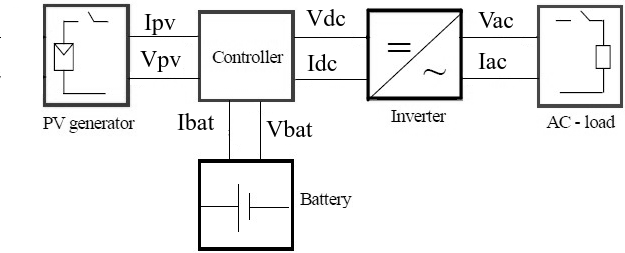
\includegraphics[width=0.5\textwidth]{blockdiagramPVS2_rev}
\centering
\caption{Block diagram for a typical stand-alone PV system~\cite{Hansen}.}
\label{fig:blockdiagram} 
\end{figure}

In this section, we explain the adopted method to size stand-alone solar PV systems, and what criteria and technique can be applied to optimal sizing. 

%%%%%%%%%%%%%%%%%%%%%%%%%%%%%%%%%%%%%%%%%%%%%%%%%%%%%%%%
\subsection{Sizing Stand-alone Solar PV Systems}
\label{sec:sizing}
%%%%%%%%%%%%%%%%%%%%%%%%%%%%%%%%%%%%%%%%%%%%%%%%%%%%%%%%

We adopted a critical period (worst month) solar energy method~\cite{Pinho}; in particular, the maximum power point tracking (MPPT) charge controller, which is the most common nowadays. Firstly, we need to correct the daily energy consumption estimated for the load ($E_{consumption}$), which is carried out by Eq.~\eqref{eq:Ecorrected}, where the efficiency of batteries ($\eta_{b}$), controller ($\eta_{c}$), and inverter ($\eta_{i}$) are considered as follows
%
\begin{equation}
\label{eq:Ecorrected}
E_{corrected} = \dfrac{E_{consumption}}{\eta_{b} \times \eta_{c} \times \eta_{i} }.
\end{equation}

We must estimate the total power that will be demanded from the PV panels, as defined by Eq.~\eqref{eq:Pminpanel}.
%
\begin{equation}
\label{eq:Pminpanel}
P_{min,panels} = \dfrac{1.25 \times E_{corrected}}{Insolation},
\end{equation}

\noindent where $Insolation$, also called solar irradiation or solar exposure, is expressed in terms of $kWh/m^{2}$ per day and depends on the site where the PV system will be deployed. A factor of $20$\% for losses is considered, because $1.25 = 1 \mathbin{/} (1 - 0.2)$.

On the one hand, the sizing must meet this requirement of minimum power supplied from the PV panels $P_{min,panels}$. On the other hand, the arrangement, if in series or parallel connections, it will depend on the charge controller specification of current ($I_{c} \geq I_{total,PVpanels}$) and voltage ($V_{c} \geq V_{total,PVpanels}$).
%
Concerning the batteries, the energy $E_{b}$ to be demanded by the PV system, in order to meet the load requirements, is defined by Eq.~\eqref{eq:Ebat}.
%
\begin{equation}
\label{eq:Ebat}
E_{b} = \dfrac{Autonomy \times E_{corrected}}{DOD},
\end{equation}

\noindent where $Autonomy$ is the number of days expected for the PV system to work even when rain or clouds avoid the recharging of batteries; it is usually a design definition, which has a value ranging from $0.5$ to $2$ days. $DOD$ is the depth of discharge or the fraction of discharge. The $DOD$ is usually $25$\% for lead-acid batteries, and $80$\% for lithium batteries; that represents a State of Charge ($SOC$) of $75$\% and $20$\% respectively, because $SOC=1-DOD$. However, it is worth separating the $DOD$ into two different definitions when the battery autonomy is larger than one day ($24$ hours). In this study, the definition given here is for a maximum of $DOD$. When we deal with daily $DOD$, we will call it $DOD_{day}$, and obviously, the sum of every $DOD_{day}$ can not exceed the maximum $DOD$.

In order to define the $DOD_{day}$, we use $DOD_{day} = \dfrac{E_{corrected} \times 100}{E_{b}}$. Moreover, the minimum current from the DC bus is defined by $I_{min,DCbus} = \dfrac{E_{b}}{V_{system}}$. Those equations are important to define the system battery arrangement (series and parallel), where $V_{system}$ is the DC voltage of the bus. 

As for batteries, we must first define the total capacity of the battery bank, which can be described as
%
\begin{equation}
\label{eq:Cbank}
C_{bank} = \dfrac{Autonomy E_{load}}{DOD \eta _{b} V_{system}},
\end{equation}

\noindent where $ E_{load} $ is the average energy consumed by the load corrected according to PV equipment efficiency, and $ \eta_{b} $ is the efficiency of the battery.
%
Eq.~\ref{eq:batcheck} then performs the final sizing check, considering the number of batteries in series ($ N_{BS} $) and the number of batteries in parallel ($ N_{BP} $) adopted as
%
\begin{equation}
\label{eq:batcheck}
\left( N_{BS} \times N_{BP} \right) \geq N_{B}total.
\end{equation}

The charge controller must initially meet the voltage requirement of the PV system, as described by
% 
\begin{equation}
\label{eq:vcvsystem}
V_{c} = V_{system}.
\end{equation}

The short circuit reference information from the manufacturer's solar panel must be corrected to the cell temperature because field temperature is higher than nominal or laboratory temperature, and the PV system is temperature dependent, as described by
%
\begin{equation}
\label{eq:iscamb}
I_{sc,amb} = \dfrac{G}{G_{ref}} \left[ I_{sc,ref} + \mu_{I} \times (T-25) \right]. 
\end{equation}

The controller must meet the maximum current from the PV array ($I_{c,min} = I_{sc,amb} \times N_{PP}$ and $I_{c} \geq I_{c,min}$).

The inverter sizing check is performed through three equations: $V_{in}DC = V_{system}$ ensures that the input voltage of the controller meets the system voltage; $V_{out}AC = V_{AC}$ ensures that the output voltage of the controller meets the AC voltage of the load, i.e., the outlet voltage. Finally, Eq.~\eqref{eq:invcheck} ensures that the controller can support the total demand of the load ($Demand$) and the surge power ($P_{surge}$), where $V_{in}DC$ is the nominal input voltage, and $V_{out}AC$ is the nominal output voltage of the inverter; $MAX_{AC,ref}$ is the peak power that the inverter can support.
%
\begin{equation}
\label{eq:invcheck} 
\left[ (Demand \leq P_{AC,ref}) \, and \, (P_{surge} \leq MAX_{AC,ref}) \right].
\end{equation}

Some inverter models allow parallel operation of more than one unit, besides the integration to create bi- and three-phase circuits. It is advisable to use pure sine wave inverters for electronic loads sensitive to harmonic distortion waves.

Besides that, it is crucial to verify the compatibility between the charge controller and inverter because some models are not compatible with equipment from other manufacturers. Furthermore, it is vital to select an inverter power that is lower than (or equal) the charge controller power, because the demand from the electric load causes the inverter to transfer this demand from the DC side (and a controller overcharge).

%All the equations model the continuous-time behavior of the PV system; they produce real numbers except for the batteries and panels, where real numbers must be converted into integer ones (it is not possible to deploy a fraction of panels or batteries). The verification and simulation tools need to handle non-linear real arithmetic to produce the result.

%%%%%%%%%%%%%%%%%%%%%%%%%%%%%%%%%
\subsection{PV Systems Optimization: Criteria and Techniques}
%%%%%%%%%%%%%%%%%%%%%%%%%%%%%%%%%

We need to evaluate \textit{power reliability} and \textit{system cost analysis} for the underlying system to select an optimal PV system to meet size constraints. %An ideal combination of any PV system consists of the best compromise between these two objectives or criteria. 
During the PV system design, one of the most important aspects to ensure power system reliability is to analyze power supply availability~\cite{Alsadi2018}. The reason is that solar energy production is intermittent and, therefore, the energy generated usually does not match with the load demand. Reliable power is a generation system that has sufficient power to feed load demand in a period. There exist different methods to express system reliability, where the most popular ones are the loss of load probability (LOLP) and the loss of power supply probability (LPSP)~\cite{Alsadi2018}. In both methods, if the probability is zero, then the load is always fulfilled; otherwise (i.e., probability of one), the load is never fulfilled. %LOLP is the probability for the case when load demand exceeds the generation power by the PV system.
On the one hand, we have a reliable PV system when it can generate sufficient power to fulfill the demanded load within a period. On the other hand, LPSP is defined as the probability of the case when the system generates insufficient power to satisfy the load demand. The main approaches to LPSP demand simulation or probabilistic treatment of time series data to predict dynamic changes in system performance. However, data is not always available, and dynamic analysis is complex; and this is a drawback of LOLP and LPSP~\cite{Alsadi2018}.

There exist various methods available related to economic analysis. The main objective is to determine whether the project has an acceptable investment; the usual way is to perform economic analysis after reliability analysis to propose a system with high reliability and lowest cost~\cite{Alsadi2018}. The conventional methods include: Net Present Cost (NPC)~\cite{Park2004}, the Levelized Cost of Energy (LCOE)~\cite{Zhou2010}, or the Life Cycle Cost (LCC)~\cite{Applasamy2011}. The NPC is the present value of all the costs over the project lifetime, minus the present value of all the revenues that it earns over the project lifetime. We find the present net worth by discounting all cash inflows and outflows, including the cost of installation, replacement, and maintenance of the PV system, at an internal rate of return (IRR)~\cite{Park2004}. IRR is used to evaluate the attractiveness of a project or investment. We define LCOE as the average cost per kWh of usable electrical energy produced by the PV system when a lifetime, investment cost, replacement, operation and maintenance, and capital cost are considered~\cite{Kamel2005}. LCOE method is useful in comparing different generation technologies with different operating characteristics~\cite{Zhou2010}. LCC is the estimation of the sum of installation cost, operating, and maintenance of a PV system for some time, and expressed in today's value~\cite{Applasamy2011}. Eq.~\eqref{eq:LCC} is used to calculate LCC of a PV system,
%
\begin{equation}
\label{eq:LCC}
\begin{aligned}
LCC = & C_{PV} + C_{bat} + C_{charger} + C_{inv} + \\
   & C_{installation} + C_{batrep} + C_{PWO\&M},
\end{aligned}
\end{equation}

\noindent where $C_{PV}$ is PV array cost, $C_{bat}$ is initial cost of batteries, $C_{charger}$ is cost of charger, $C_{inv}$ is inverter cost, $C_{installation}$ is installation cost, $C_{batrep}$ is battery replacement cost in present value, and $C_{PWO\&M}$ is operation and maintenance costs in present worth.

Parallel to criteria, the designer has to evaluate the design based on optimization variables to recommend an optimal configuration for PV systems. As the number of optimization variables increases, the computational effort increases as well. Hence, to obtain the best PV system design as well as a simplified sizing process, prior work introduced three primary techniques for system sizing calculation, namely intuitive, numerical, and analytical methods~\cite{Zhou2010}. The intuitive method is simple, easy to be implemented, and can be used to give rough suggestions for preliminary design. The sizing rules rely on the designer's experience, using the lowest performance either in a time data or by directly using average value (daily, monthly, or annual) of solar irradiance. This method does not consider the battery's state of charge or even the random nature of solar irradiation and meteorological conditions~\cite{Alsadi2018}. For the numerical method, the design simulates for each time step within a period to calculate and investigate the state of charge of batteries. The numerical method is very accurate; however, it is complex, demanding more time for calculation~\cite{Park2004}. Analytical methods are used to obtain a close relation or correlation in the form of an equation between capacities and reliabilities. The sizing task becomes much more straightforward than the numerical technique. However, the relation cannot be applied to different sites since it is specific to one place of deployment of the PV system, thereby demanding adaptation if another site is analyzed.

%------------------------------------------------------
\section{Automated Formal Synthesis Method}
\label{sec:Method}
%------------------------------------------------------

In this section, we present our methodology to obtain the optimal sizing of stand-alone solar PV systems through program synthesis. Fig.~\ref{fig:optimization} illustrates how to obtain the optimal sizing of a stand-alone PV system, which shows the traditional techniques (manual and simulation) and the proposed automated synthesis. Note that the input information is the same for all the methods: weather data, price information, design requirements, as load curve and power demand, and design assumptions, except for the automated synthesis, where we also define the bound $k$ to restrict the design-space search. Concerning the output presented by both techniques, all of them produce a successful or fail result considering a feasible technical solution with the lowest cost. On the one hand, when done by simulation, we get a report or graphical result; on the other hand, the automated synthesis technique, which is mathematical reasoning of a model, presents a counterexample with the optimal solution stored in variables. Furthermore, the design-space coverage during the optimal sizing search is sound and complete when using automated synthesis.
%
\begin{figure}[h]
%\hspace*{-1cm} 
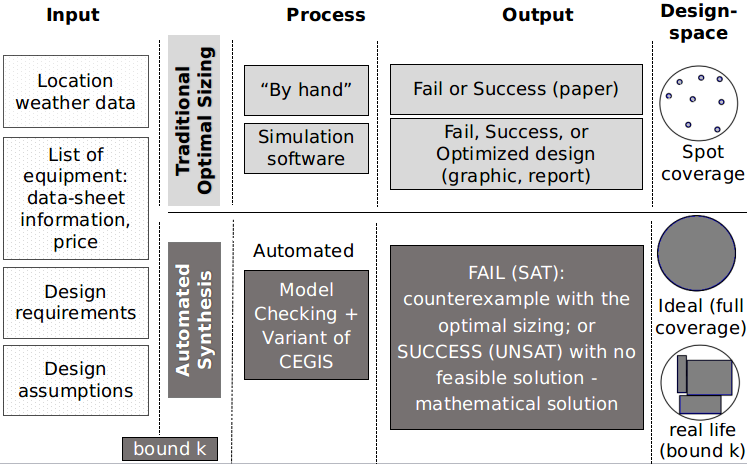
\includegraphics[width=0.51\textwidth]{optimalsizingprocess4}
\centering
\caption{Comparative of optimal sizing methods.}
\label{fig:optimization}
\end{figure}

%%%%%%%%%%%%%%%%%%%%%%%%%%%%%%%%%%
\subsection{Automated Verification Using Model Checking}
\label{sec:AutomatedVerification}
%%%%%%%%%%%%%%%%%%%%%%%%%%%%%%%%%%

%Although simulation and testing explore possible behaviors and scenarios of a given system, they leave open the question of whether new trajectories may contain a flaw. Formal verification conducts an exhaustive exploration of all possible behaviors; when a design is said to be ``correct'' by a formal verification method, it implies all behaviors explored, and questions regarding adequate coverage or missed behavior become irrelevant~\cite{Clarke2012}. Formal verification is a systematic approach that applies mathematical reasoning to obtain guarantees about the correctness of a system; one successful method in this domain is \textit{model checking}~\cite{Clarke2012}. 

To perform the automated formal synthesis, we use a state-of-the-art model checker. ESBMC (or Efficient SMT-based Bounded Model Checker) is a bounded and unbounded model checker for C programs~\cite{esbmc2018}, which supports the verification of LTL properties with bounded traces~\cite{DBLP:journals/sosym/MorseCN015}. ESBMC's verification flow can be summarized in three stages: (i) a front-end that can read and compile C code, where the formal system specification is first handled; (ii) preprocessing steps to deal with code representation, control flow and unwinding of loops, and model simplification, thereby aiming to reduce verification effort; and finally (iii) the SMT solving stage, where all constraints and properties of the system are encoded into SMT and checked for satisfiability. ESBMC exploits the standardized input language of SMT solvers (SMT-LIB\footnote{\url{http://smtlib.cs.uiowa.edu/}} logic format) to make use of a resource called \textit{assertion stack}~\cite{Morse2015}. This enables ESBMC, and the respective solver, to learn from previous checks, thus optimizing the search procedure and potentially eliminating a large amount of the formula state-space to be searched, because it solves and disregards data during the process, incrementally. This technique is called ``incremental SMT''~\cite{DBLP:journals/fac/SchrammelKBMTB17} and it reduces the memory needed, helping to deal with the entire design space state.

%However, there exists a main disadvantage of model checking: the state explosion problem~\cite{Clarke2012}. In order to solve this issue, many different techniques were developed at the last decades. One of the promising is the Bounded Model Checking (BMC). BMC algorithms traverses a finite state machine for a fixed number of steps, $k$, and checks whether violation occurs with this bound. 
%The CPA framework provides interfaces to SMT (Satisfiability Modulo Theories) solvers and interpolation procedures~\cite{Beyer2011}. Currently, CPAchecker uses MathSAT as SMT solver~\cite{Beyer2011}. The use of SMT by CPAchecker, instead of Boolean Satisfiability SAT from the original BMC, comes as an alternative to overcome limitations of the systems modeling, especially considering that the complexity of these is increasing and the SMT method has high level and richer theories than the SAT to represent the models.
%
%-----------------------------------------------------------
\subsection{Program Synthesis Technique}
\label{sec:ProgramSynthesis}
%-----------------------------------------------------------

%Program synthesis addresses an age-old problem in computer science: can a computer program itself?~\cite{Bornholt2019}. Before the computer can automatically generate a program, it is necessary to give it a specification of what the program should do. The specification needs to describe the program's desired behavior to ensure that the program does what it intends.
The basic idea of program synthesis is to automatically construct a program $P$ that satisfies a correctness specification $\sigma$. In particular, program synthesis is automatically performed by engines that use a correctness specification $\sigma$, as a starting point, and then incrementally produce a sequence of candidate solutions that partially satisfy $\sigma$~\cite{Abateetal2017}. As a result, a given candidate program $p$ is iteratively refined to match $\sigma$ more closely. CEGIS represents one of the most popular approaches to program synthesis currently used in practice for cyber-physical systems~\cite{Abateetal2017}. %, as energy production, distribution, and optimization. 
Figure~\ref{Counter-Example-Guided-Inductive-Synthesis} illustrates the architecture. 
%Note that CEGIS has close connections to algorithmic debugging using counterexamples and abstraction refinement~\cite{Alur}. %from model checking.
%
\begin{figure}[h]
	\centering
%	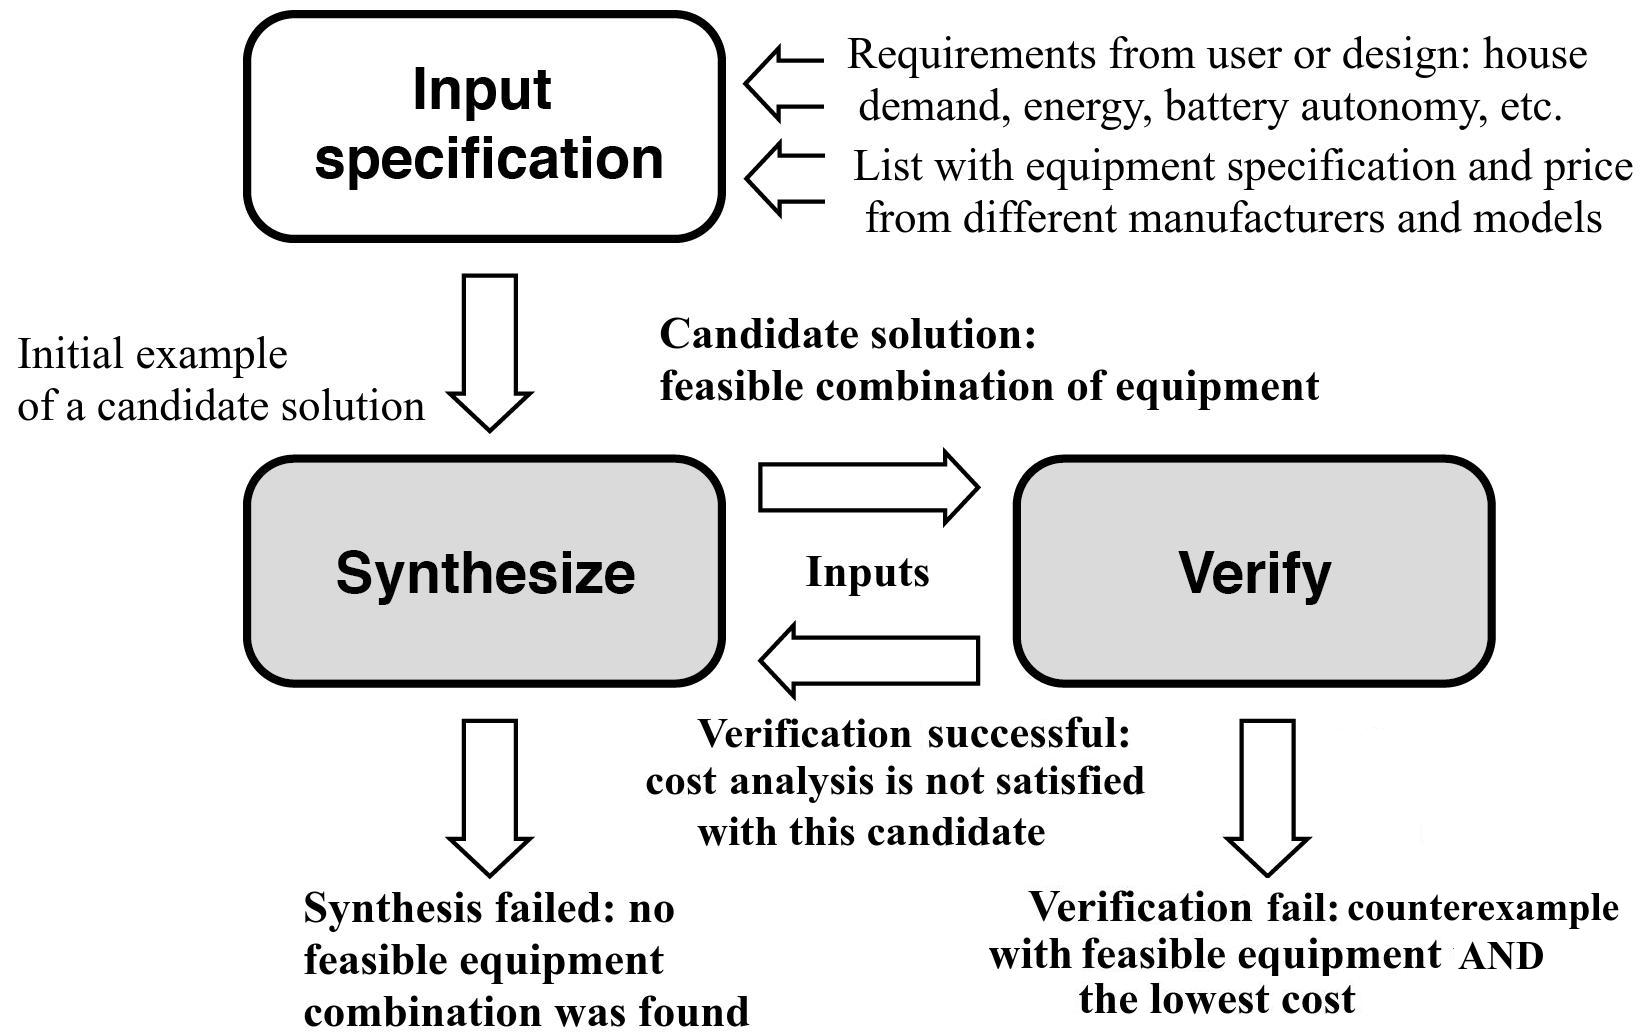
\includegraphics[width=0.75\columnwidth]{fig2_rev2.jpg}
	\hspace*{-1cm}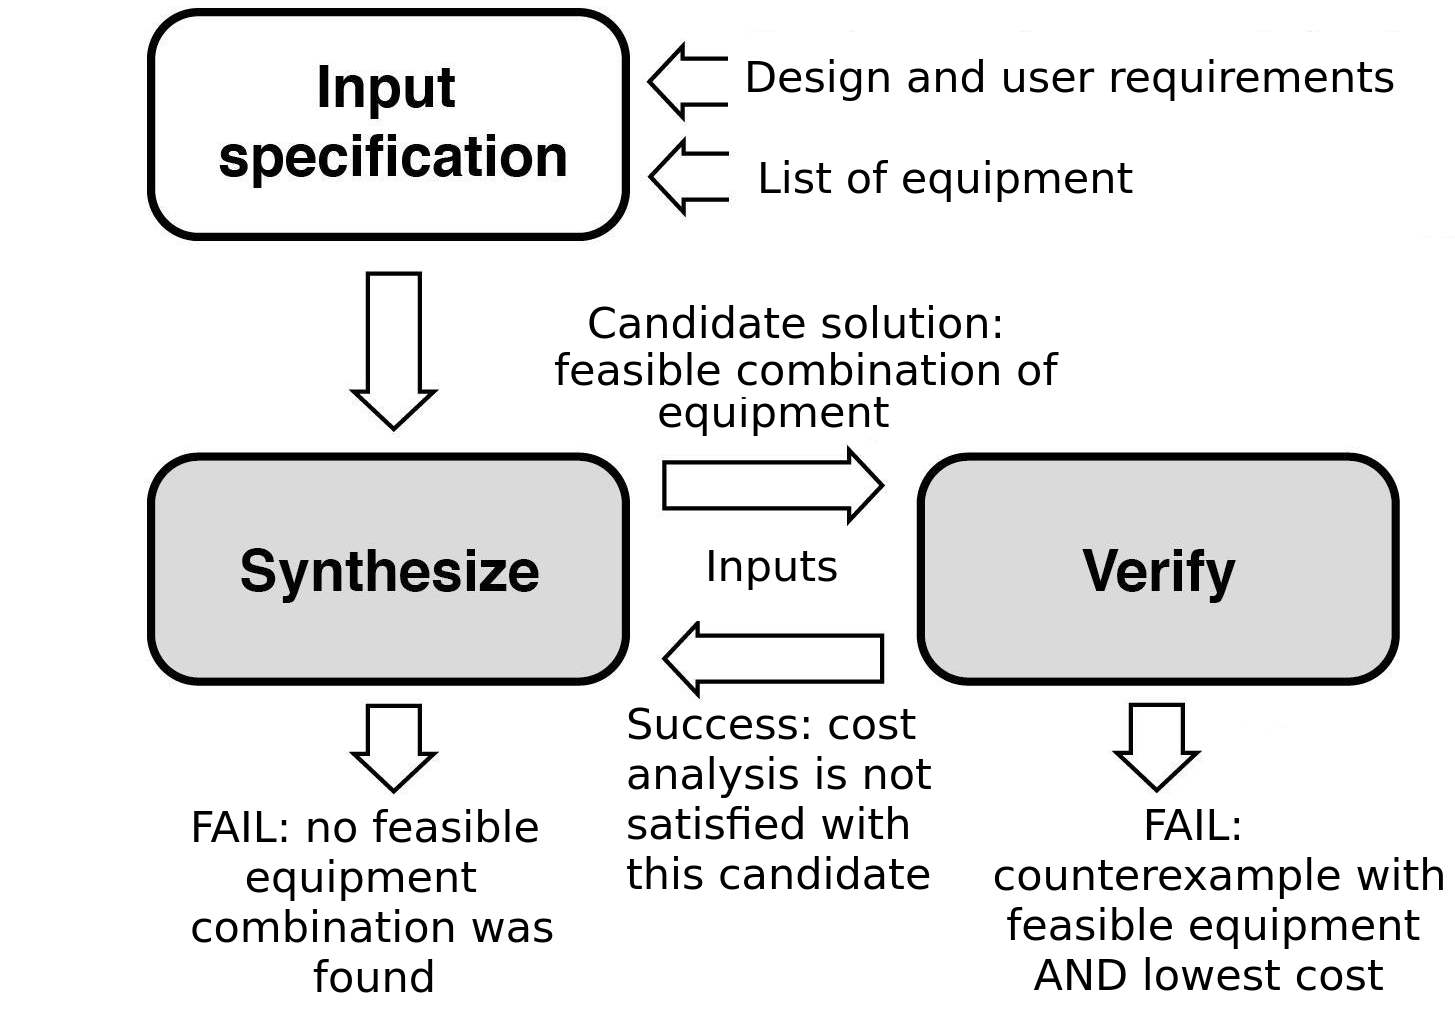
\includegraphics[width=0.5\textwidth]{fig2_rev4}
	\caption{CEGIS adapted to PV system sizing.}
	\label{Counter-Example-Guided-Inductive-Synthesis}
\end{figure}

The correctness specification $\sigma$ provided to our program synthesizer is of the form $\exists \vec{F} . \forall \vec{x}. \sigma(\vec{x}, \vec{F})$, where $\vec{F}$ ranges over functions, $\vec{x}$ ranges over ground terms, and $\sigma$ is a quantifier-free (QF) formula typically supported by SMT solvers. The ground terms are interpreted over some finite domain $\mathcal{D}$, where $\mathcal{D}$ can be encoded using the SMT's bit-vectors part. Examples of specifications used by our method include house demand, energy, and battery autonomy; we also provide a list of equipment specifications and prices from different manufacturers and models.

In Figure~\ref{Counter-Example-Guided-Inductive-Synthesis}, regarding traditional CEGIS method~\cite{AbateCAV2018}, the phases {\sc Synthesize} and {\sc Verify} interact via a finite set of test vectors {\sc inputs}, which is incrementally updated. Given the correctness specification $\sigma$, the {\sc Synthesize} procedure tries to find an existential witness $\vec{F}$ satisfying the specification $\sigma(\vec{x}, \vec{F})$, for all $\vec{x}$ in {\sc inputs} (as opposed to all $\vec{x} \in \mathcal{D}$). If {\sc Synthesize} succeeds in finding a witness~$\vec{F}$, the latter is a candidate solution (i.e., feasible combination of equipment) to the full synthesis formula, which is passed to {\sc Verify} in order to check whether it is a proper solution ({\it i.e.}, $\vec{F}$ satisfies the specification $\sigma(\vec{x}, \vec{F})$ for all $\vec{x}\in\mathcal{D}$). If this is the case, then the algorithm terminates, i.e., we have found a feasible equipment with the lowest cost; otherwise, in the CEGIS traditional method, additional information is provided to the phase {\sc Synthesize}, in the form of a new counterexample that is added to the {\sc inputs} set and the loop iterates again.

One may notice that each iteration of the traditional CEGIS loop adds a new input to the finite set $\text{\sc inputs}$, which is then used for synthesis. Given that the full set of inputs $\mathcal{D}$ is finite because we use bit-vector expressions, this means that the refinement loop can only iterate over a finite number of times. However, {\sc Synthesize} may conclude that no candidate solution obeying $\sigma$ for the finite set $\text{\sc inputs}$ exists, and our synthesis engine can then conclude that no possible equipment combination was found.

In our variant CEGIS method, there exist four distinct differences related to the traditional CEGIS: 
(1) there exists no test vector, and every candidate is generated during the run-time in the {\sc Synthesize} phase and sent to the {\sc Verify} phase; 
(2) if the {\sc Verify} phase is unsuccessful, then a new candidate is generated by {\sc Synthesize} and 
(3) the lower bound of the {\sc Verify} phase is incremented to search for the lowest cost; 
(4) as a result, there exists no refinement from the {\sc Verify} phase back to the {\sc Synthesize} phase, i.e., 
a new counterexample is not added to the {\sc input} set since a failure during the {\sc Verify} phase will only discard a given candidate, which could be feasible in the next iteration with a new lower bound.

Program synthesis engines that implement the CEGIS approach~\cite{sketch} can automatically produce solutions for a large variety of specifications; here, we have used symbolic software verifiers based on SMT solvers.
%
Algorithm~\ref{alg:verification-algorithm} describes our pseudo-code to synthesize stand-alone PV systems using symbolic model checking. We adopted the analytical method of optimization, with LCC economic analysis and power reliability based on the worst month criteria.

 \begin{algorithm}
 \caption{Synthesis algorithm}
 \begin{algorithmic}[1]
 \begin{scriptsize}
 \renewcommand{\algorithmicrequire}{\textbf{Input:}}
 \renewcommand{\algorithmicensure}{\textbf{Output:}}
 \REQUIRE weather data (temperature, solar irradiance); data from panels, controllers, batteries, and inverters; design requirements (load curve, peak demand, load surge power, energy consumption, battery autonomy, AC voltage); design assumptions (SOC, DOD, criteria and objectives for technical and cost analysis)
 \ENSURE FAIL (SAT) with counterexample showing the optimal sizing; SUCCESS (UNSAT), saying that the project has no feasible solution considering the requirements and the list of equipment
 \STATE Initialize variables \\
 \STATE Declare the maximum possible cost $MaxCost$ \\
 \STATE Calculate min possible Cost $MinCost$, based on the equipment list \\
 \FOR {$HintCost=MinCost$ to $MaxCost$} 
 	\STATE Declare non-deterministic variables to select PV Panel, Controller, Battery, and Inverter from list \\
 	\STATE Calculate $E_{corrected}, \, P_{min,panels} $ \\
	\STATE Calculate and define PV panels arrangement $N_{TP}, \, N_{PS}, N_{PP} $ \\
	\STATE Requirement enforced by \textbf{assume}$(P_{min,panels} \leq (N_{PS} \times N_{PP} \times P_{m,ref}))$ \\
	\STATE Calculate $I_{c,min} = N_{PP} \times I_{m,ref}$ \\
	\STATE Calculate $V_{c,min} = N_{PS} \times V_{m,ref}$ \\
 	\STATE Calculate $C_{bank}$ and $E_{b}$ \\
	\STATE Calculate and define battery arrangement $N_{BS}, \, N_{BP}, \, N_{BTotal}$ \\
	\STATE Requirement enforced by \textbf{assume} $(I_{min,DCbus} \leq (N_{BP} \times Capacity))$ \\
 	\STATE Controller requirements enforced by \textbf{assume}$((P_{controller} \geq P_{inverter}) \wedge V_{c} \wedge I_{c})$ \\
	\STATE Inverter requirements enforced by \textbf{assume}$(V_{in}DC \wedge V_{out}AC \wedge Demand \wedge P_{surge})$ \\
	\STATE non-deterministic variables hold feasible equipment and cost \\
	\STATE $F_{obj} \leftarrow N_{TP}*Panel_{Cost} \, + \, N_{TB}*Battery_{Cost} \, + Controller_{Cost} \, + \, Inverter_{Cost} \, + \, Installation_{Cost} \, + \, batrep_{Cost} \, + \, PWO\&M_{Cost}$ \\
	\STATE Violation check with \textbf{assert}$(F_{obj} > HintCost)$ \\
 \ENDFOR
 \RETURN $(\,)$ 
 \end{scriptsize}
 \end{algorithmic} 
 \label{alg:verification-algorithm}
 \end{algorithm}

Our synthesis algorithm will synthesize constant values; it starts with the input of the manufacturer's data and prices of PV panels, batteries, charge controllers, and inverters. Moreover, we define design (house) requirements and design assumptions. 
%
The \textit{for}-loop started in line $4$ controls the lowest cost of the PV solution. In particular, it starts with cost $MinCost$ and stops when the algorithm finds a feasible solution in which the cost breaks the $assertion$ stated in line $18$. If that happens, then our algorithm has found an optimal solution, thereby stating that the {\sc Verify} phase reached a satisfiable condition (\textit{SAT}). The $MaxCost$ value in line $2$ is just a very high value inserted as a limit to the \textit{for}-loop, which has two properties. (1) It will never be reached because the optimal solution will be found first (SAT result) or (2) it will be reached when the search engine did not find a feasible solution for the optimization (UNSAT result).

Our synthesis algorithm uses non-deterministic variables to choose one specific constant from a given list of PV panels, controllers, batteries, and inverters (line $5$). This procedure ensures that our synthesis engine checks all combinations of items from each equipment, and combines them to assemble a viable (candidate) PV solution, which meets user requirements. A list of forty equipment from ten different manufacturers was provided (as INPUT) to our synthesis engine to allow the choice of every item of PV sizing. Data-sheet from each item was necessary to collect technical information.\footnote{\url{http://tiny.cc/4ny4nz}} Moreover, the price of each item was obtained from available quotations in the market in US dollars. %, and if the currency was not in US dollars, then it was used the exchange rate of the day to convert it to US dollars. %All this data is available online\footnote{\url{https://drive.google.com/file/d/1DUtM3Ui\_pU54DmtTXnW1DUcanOcXBVeg/view?usp=sharing}}.

Next, we use from Eq.~\eqref{eq:Ecorrected} to Eq.~\eqref{eq:invcheck} to calculate the sizing variables (lines $9$ to $15$). The directive \textit{assume} (lines $8$, $13$, $14$, and $15$) ensures compatibility of the items chosen from the list of equipment: the {\sc Verify} phase uses only items (among all the possible ones) that satisfy the statements of those lines. Line $5$ is specific to PV panels. Line $13$ is for the battery bank. Line $14$ is the charge controller voltage check. Line $15$ does the inverter check and ensures the power demand and the inverter surge power.
Our algorithm reaches line $16$ with one feasible solution, and the cost of that solution is calculated in $F_{obj}$ (line $17$). This cost is the equivalent to Eq.~\eqref{eq:LCC}.

If our algorithm does not find a feasible solution among the item of equipment that was provided for our {\sc Synthesize} phase, then the result is unsatisfiable (\textit{UNSAT}). In particular, the program finishes without finding a solution, indicating that it was unable to combine the specific items of equipment to create a feasible solution. 
%
The main challenge for the {\sc Synthesize} phase is to find a feasible candidate solution for the constraints and user requirements. The challenge for the {\sc Verify} phase is to find the lowest acquisition cost from a list of equipment and components provided by the {\sc Synthesize} phase. 
%
Note that the process is completely automated and that validation is performed by our {\sc Verify} phase to ensure that the solution is sound.
Algorithm~\ref{alg:verification-algorithm} is transformed by the verification engines into the Boolean expressions, which are passed to the solver to verify ($C \wedge \neg P$), as shown online.\footnote{\url{http://tiny.cc/ity4nz}}

%%%%%%%%%%%%%%%%%%%%%%%%%%%%%%%
\subsection{Assumptions and Premises}
%%%%%%%%%%%%%%%%%%%%%%%%%%%%%%%
%
%Regarding the line $2$ of Algorithm~\ref{alg:verification-algorithm}, a list of forty equipment from ten different manufacturers was provided to our synthesis engine in order to allow the choice of every item of PV sizing. Data sheet from each item was necessary to collect technical information. Moreover, the price of each item was obtained from available quotations in the market, and if the currency was not in US dollars, then it was used the exchange rate of the day to convert it to US dollars. %All this data is available online\footnote{\url{https://drive.google.com/file/d/1XOQMC0zdybvTLyBLo-TlChLdwDFUlUCT/view?usp=sharing}}.

Concerning power reliability, this work will rely on the critical period solar energy method~\cite{Pinho}, as described in Section~\ref{sec:sizing}.  %The usual way is to use LOLP or LPSP. However, we are neither considering site characteristics nor the load changes over time, which demands historical data. The reliability analysis will be developed only by the critical period method of PV sizing.
%
Regarding financial analysis:
\begin{itemize}
	\item \textit{LCC lifetime considered}: $20$ years;
	\item \textit{Installation costs}: includes delivery in the isolated community and installation costs itself, $5$\% of total cost~\cite{Agrener2013};
	\item \textit{Discount or interest rate value}: $10$\%, which is a good rate considering financial investments in developing countries;
	\item \textit{Operation and maintenance annual costs}: based on PV projects of similar size in the Amazon region of Brazil, we will adopt US\$ 289.64~\cite{Agrener2013}. This cost includes the battery replacement based on its lifetime, plus inverters and controller replacement (every $10$ year). We adopted lead-acid batteries, the cheapest and most common kind used nowadays; and it means a $4$ year lifetime. Therefore, it will be performed three battery bank and one inverter-controller replacements during the LCC analysis. Note that those data can be adjusted in our algorithm.
\end{itemize}

On the subject of PV system optimization technique, we will adopt here the intuitive method since the average value daily of solar irradiance is used in the mathematical model,  without considering the battery's state of charge, or even the random nature of solar irradiation and meteorological conditions. Therefore, all the computational effort will be concentrated in our automated synthesis algorithm.

Regarding all case studies, it was defined that the minimum state of charge of batteries is $75$\% (with DOD maximum of $25$\%, which is commonly adopted for lead-acid batteries), the system voltage is set in $24$ V DC (the most common as well, but the value can be adjusted to $12$ or $48$ V at the code), and the AC voltage from the inverter is $127$ V (Brazilian standard).

Related to off-the-shelf simulation tools, only HOMER Pro performs off-grid systems with battery backup analysis and includes economical analysis. Therefore, in this study, HOMER Pro will be the simulation tool used to compare with our automated synthesis method. Related to HOMER Pro: (a) is available only for Microsoft Windows, and its annual standard subscription costs US\$ $504.00$~\cite{HOMER}; (b) it does not have the LCC cost in its reports. It has NPC and LCOE. Therefore NPC was used to obtain LCC in order to allow the comparative; (c) the optimization analysis of HOMER allows us to define a load curve and temperature according to data collected from online databases. However, in order to allow a correct comparative, the curve load and the temperature were defined the same as automated synthesis tools; (d) it does not have explicit equipment called a charge controller. It uses a controller resource that can perform in two different ways, according to the optimization choice or the user choice: load following or cycle charging~\cite{HOMER}. During the tests, it was chosen the load following controller: it produces only enough power to meet the demand~\cite{HOMER}; (e) It was assumed the value of 5\% of capacity shortage that is equivalent to 95\% of availability of the PV system. By definition, availability is the percentage of time at which a power system is capable of meeting the load requirements~\cite{Khatib2014}. For critical loads, 99\% is considered acceptable. While in an ordinary house electrical load, 95\% is considered acceptable; (f) it was assumed a string of two batteries in order to match the voltage of the system of $24$ V DC that was used for the automated synthesis tool; (g) the premise adopted when using HOMER Pro it was that the user does not know the optimal solution and that in order to obtain this solution is necessary to include (at the design phase of the tool) generic PV and batteries modules that HOMER will search for the optimized power of each component. With that in mind, it was included a generic flat-plate PV of $1$ kW and generic lead-acid batteries of $1$ kW as well (and with the capacity of $83.4$ Ah according to HOMER Pro modeling). HOMER, during run-time, decides the size in kW of each module, based on feasibility and lower cost.

%---------------------------------------------------------------------------
\section{Case Studies and Analysis}
\label{sec:Results}
%---------------------------------------------------------------------------

This section describes our case studies, experimental set-up, and results to evaluate our proposed synthesis approach. We compare our approach with a specialized optimization tool.

%---------------------------------------------------------------------------
\subsection{Case studies} 
%---------------------------------------------------------------------------

We have performed seven case studies to evaluate our proposed synthesis approach, as described in the first column of Table~\ref{tab1} (\textit{Specification}). These case studies were defined based on real houses visited by the team of a Newton Fund project in 14 riverside communities.\footnote{\url{http://star-energy.coventry.ac.uk/}} For all cases, an estimated load curve (kWh) was defined based on the electronics consumers found into each house.

\begin{table}
\caption{Case studies and results: optimization of PV systems.}\label{tab1}
\begin{scriptsize}
\begin{tabular}{c|c|c}
\hline
\hline
Tools & \makecell{ESBMC 6.0.0 \\(Boolector 3.0.1)}& HOMER Pro 3.13.1\\
\hline
\hline
Specification & Result & Result\\
\hline
\makecell{\textbf{Case Study 1}\\Peak:342W\\Surge:342W \\E:3,900Wh/day\\Autonomy:48h} & \makecell{SAT (620 min) \\NTP:6$\times$330W (2P-3S)\\NBT:16$\times$105Ah (2S-8P)\\Controller 35A/145V\\Inverter 700W/48V\\LCC: US\$ 10,214.04} & \makecell{(Time: 0.33 min)\\2.53 kW of PV\\NBT:12$\times$83.4Ah (2S-6P)\\0.351kW inverter\\LCC: US\$ 7,808.04}\\
\hline
\makecell{\textbf{Case Study 2}\\Peak:814W\\Surge:980W\\E:4,880Wh/day\\Autonomy:48h} & TO & \makecell{(Time: 0.18 min)\\3.71 kW of PV\\NBT:20$\times$83.4Ah (2S-10P)\\0.817kW inverter\\LCC: US\$ 12,861.75} \\
\hline
\makecell{\textbf{Case Study 3}\\Peak:815W\\Surge:980W\\E:4,880Wh/day\\Autonomy:12h} & \makecell{SAT (63 min) \\NTP:14$\times$150W (7P-2S)\\NBT:6$\times$105Ah (2S-3P)\\Controller 35A/145V\\Inverter 1,200W/48V\\LCC: US\$ 9,274.07} & Not possible \\
\hline
\makecell{\textbf{Case Study 4}\\Peak:253W\\Surge:722W\\E:3,600Wh/day\\Autonomy:48h} & \makecell{SAT (147 min) \\NTP:6$\times$330W (2P-3S)\\NBT:16$\times$105Ah (2S-8P)\\Controller 35A/145V\\Inverter 280W/48V\\LCC: US\$ 9,678.63} & \makecell{(Time: 0.23 min)\\2.42 kW of PV\\NBT:12$\times$83.4Ah (2S-6P)\\0.254kW inverter\\LCC: US\$ 7,677.95}\\
\hline
\makecell{\textbf{Case Study 5}\\Peak:263W\\Surge:732W\\E:2,500Wh/day\\Autonomy:48h} &  \makecell {SAT (36.70 min) \\NTP:4$\times$330W (2S-2P)\\NBT:14$\times$80Ah (2S-7P)\\Controller 35A/145V\\Inverter 280W/24V \\LCC: US\$ 8,900.70} & \makecell{(Time: 0.18 min)\\1.59 kW of PV\\NBT:10$\times$83.4Ah (2S-5P)\\0.268kW inverter\\LCC: US\$ 6,175.57} \\
\hline
\makecell{\textbf{Case Study 6}\\Peak:322W\\Surge:896W\\E:4,300Wh/day\\Autonomy:48h} &  \makecell {SAT (380.93 min) \\NTP:6$\times$320W (2P-3S)\\NBT:18$\times$105Ah (2S-9P)\\Controller 35A/145V\\Inverter 400W/24V \\LCC: US\$ 10,136.61} & \makecell{(Time: 0.22 min)\\3.15 kW of PV\\NBT:14$\times$83.4Ah (2S-7P)\\0.328kW inverter\\LCC: US\$ 9,112.45} \\
\hline
\makecell{\textbf{Case Study 7}\\Peak:1,586W\\Surge:2,900W\\E:14,000Wh/day\\Autonomy:48h} & UNSAT (0.48 min) & \makecell{(Time: 0.20 min)\\12.5 kW of PV\\NBT:66$\times$83.4Ah (2S-33P)\\1.60kW inverter\\LCC: US\$ 41,878.11} \\
\hline
\hline
\end{tabular}
\\Legend: TO= time out; E= energy; NTP= total number of panels, NBtotal= total number of batteries, NPS= number of panels in series; NPP= number of panels in parallel, NBS= number of batteries in series; NBP= number of batteries in parallel; LCC= Life Cycle Cost.
\end{scriptsize}
\end{table}

%---------------------------------------------------------------------------
\subsection{Set-up and Objectives} 
%---------------------------------------------------------------------------

The state-of-art verification tool ESBMC\footnote{Command-line: \$ esbmc filename.c -\phantom{}-incremental-bmc -\phantom{}-boolector} v6.0.0~\cite{esbmc2018} with the Boolector 3.0.1 solver~\cite{Brummayer} was used as our reference verification engine. The optimization tool HOMER Pro version $3.13.1$ was used for comparative purposes. The optimal sizing produced by ESBMC and HOMER Pro were validated with PVsyst v$6.86$~\cite{PVsyst}. PVsyst is an MS-Windows software used for the study, sizing, simulation, and data analysis of solar PV systems, with a comprehensive list of commercial equipment. PVsyst does not perform optimization. % nor does it have commercial inverter equipment.

Our evaluation aims to answer two experimental questions: [\textbf{EQ1}] \textbf{(soundness and completeness)} does our automated synthesis approach provide correct results? [\textbf{EQ2}] \textbf{(performance)} how does our formal synthesis tool compare to a specialized optimization tool?

All experiments regarding the verification tools were conducted on an otherwise idle Intel Xeon CPU E5-4617 ($8$-cores) with $2.90$ GHz and $64$ GB of RAM, running Ubuntu $16.04$ LTS $64$-bits. For HOMER Pro and PVsyst, we have used an Intel Core i5-$4210$ ($4$-cores), with $1.7$ GHz and $4$ GB of RAM, running Windows 10. Our experiments were performed with a predefined time out of $660$ minutes.


%---------------------------------------------------------------------------
\subsection{Results}  
%---------------------------------------------------------------------------
ESBMC was able to reach the optimal sizing of case studies $1$, $3$, $4$, $5$, and $6$ with a FAIL/SAT response, varying from $36$ minutes to $10$ hours. ESBMC, with this configuration, was unable to obtain an optimal solution in cases $2$ and $7$. Case $2$ produced a \textit{time out}. Moreover, case $7$ resulted in a UNSAT result, i.e., ESBMC was unable to provide a feasible solution. However, this is not a bug, and it means that the available list of equipment can not produce a feasible solution that satisfies electrical compatibility or design requirements. This UNSAT situation was reached in less than one minute. %These experimental results answer the \textit{EQ2}.

HOMER Pro was able to evaluate six case studies (cases $1$, $2$, $4$, $5$, $6$, and $7$) under $30$ seconds; it was much faster than the proposed automated synthesis tool. Case study $3$ could not be simulated since HOMER Pro does not have the battery autonomy adjustment feature, i.e., the tool always tries to feed the given load with electricity $365$ days/year. Some HOMER Pro drawbacks were also noted. (1) System equipment does not include an explicit charge controller. HOMER Pro includes a controller automatically to simulate the charge/discharge of batteries and to meet the load requirement. However, without costs or even with electrical characteristics such as maximum current and voltage, which are common during PV sizing. (2) HOMER Pro requires the inclusion of some battery specification to initiate optimization; however, it does not change the electrical specifications during simulation; the results presented are multiples of the original battery type suggested by the user. For example, it was started with a $83.4$ Ah lead-acid battery, and during simulation, HOMER Pro did not try to use other capacities or types. (3) HOMER Pro does not present the optimal solution in terms of connections of PV panel arrays, just the total in terms of power, i.e., it presents neither the models and the power of each PV panel nor the total of panels in series or parallel.

%The authors have real PV systems deployed since June $2018$ in a riverside community in the State of Amazonas, Brazil, GPS coordinates 2$^{o}$44'50.0"S 60$^{o}$25'47.8"W, with demands of case studies $1$, $4$, $5$, and $6$, always with a $3$ $\times$ $325$ W ($3$S, total $975$ W) panels and $4$ $\times$ $220$ Ah ($2$S-$2$P $= 440$ Ah) lead-acid batteries.
%
If we compare the results of the formal synthesis against those of HOMER Pro, we observed some different results in terms of the technical solution and cost (cf. Table~\ref{tab1}). Concerning the performance, there exists a vast difference in favor of HOMER Pro that obtained the results in considerably less time: few seconds in the opposite of an average of $4$ hours for the automated synthesis technique.Particularly in the case of LCC, the cost varied from $11$\% to $44$\%, producing a higher estimation from the automated synthesis technique. However, considering that the cost of individual items of each database used to compose the optimal design is not the same among the tools, it is plausible to obtain different results.

On the one hand, concerning the PV panels sizing, the results presented by the automated synthesis were smaller in terms of power than the ones produced by the simulation tool. The difference varied from $19$\% to $65$\%. On the other hand, concerning the battery bank, the results were smaller in terms of capacity for HOMER Pro. The difference was between $34$\% to $68$\%. The mathematical models are different and particular parameters can be tuned for each technique; that can justify the difference, which was presented in all the case studies.

Related to the inverters, HOMER Pro suggests a value in kW that is very close to the maximum load of every case study, but it is not commercial value. The proposed synthesis tool, however, presents inverters that are commercial and can be obtained off-the-shelf. Our synthesis approach considers surge power demand from the house, which is not considered by HOMER Pro. This feature is a definite advantage of the formal synthesis method. HOMER Pro does not include charge controllers as a specific item of equipment in its mathematical model; only our approach presents a commercial controller and includes it during the cost analysis. Our approach, therefore, presents more reliable results than HOMER Pro.

The discrepancies between the two approaches are not easy to address without some real systems validation. We use the simulation software PVsyst to validate the optimal sizing produced, as shown in Table~\ref{tab2}. Note that PVsyst has a pre-sizing feature, which presents a minimum recommended sizing of PV panels and batteries (only), but without using manufacturers' data or models for it. This feature was used as reference mainly with HOMER Pro, where there exists no equipment brands or models (only power and capacities specification). PVsyst full feature of sizing validation was used only with the formal synthesis optimal sizing, where brands and models were simulated in PVsyst according to the sized system produced by ESBMC.

\begin{table}
\caption{Optimal sizing validation with PVsyst.}
\label{tab2}
\begin{scriptsize}
\begin{tabular}{c|c|c|c}
\hline
\hline
\makecell{Case\\Study} & \makecell{PVsyst\\(pre-sizing)}&\makecell{Formal synthesis\\optimal sizing\\validation}& \makecell{HOMER Pro\\optimal sizing\\validation}\\
\hline
\hline
\# 1 & \makecell{P= 1,166 W\\B= 381 Ah\\(minimum)}&\makecell{No error found \\100\% of avail.} & \makecell{No error found\\Panels oversized: 2.16$\times$\\Batteries oversized: 1.39$\times$}\\
\hline
\# 2 & \makecell{P= 1,482 W\\B= 478 Ah\\(minimum)}&\makecell{NA \\(TO result\\in Table~\ref{tab1})} & \makecell{No error found\\Panels oversized: 2.6$\times$\\Batteries oversized: 1.74$\times$}\\
\hline
\# 3 & \makecell{Not possible to \\simulate\\(autonomy $<$ 24h)} &\makecell{Only technique that\\produced solution} & \makecell{NA\\(autonomy $<$ 24h)}\\
\hline
\# 4 & \makecell{P= 1,078 W\\B= 354 Ah\\(minimum)}&\makecell{No error found \\97.37\% of avail.} & \makecell{No error found\\Panels oversized: 2.24$\times$\\Batteries oversized: 1.41$\times$}\\
\hline
\# 5 & \makecell{P= 823 W\\B= 268 Ah\\(minimum)}&\makecell{No error found \\100\% of avail.} & \makecell{No error found\\Panels oversized: 1.93$\times$\\Batteries oversized:  1.56$\times$}\\
\hline
\# 6 & \makecell{P= 1,299 W\\B= 421 Ah\\(minimum)}&\makecell{No error found \\100\% of avail.} & \makecell{No error found\\Panels oversized: 2.42$\times$\\Batteries oversized: 1.38$\times$}\\
\hline
\# 7 & \makecell{P= 4,263 W\\B= 1,384 Ah\\(minimum)}&\makecell{NA \\(UNSAT result\\in Table~\ref{tab1})} & \makecell{No error found\\Panels oversized: 2.9$\times$\\Batteries oversized: 1.99$\times$}\\
\hline
\hline
\end{tabular}
\\Legend: NA = sizing not available for validation; B = batteries capacity; P = panels power; Avail.= Availability (expected of 95\% or greater).
\end{scriptsize}
\end{table}

Each simulation with PVsyst took $4$ seconds. We were unable to validate case study $3$ using PVsyst since the battery autonomy is less than 24 hours, and only the proposed synthesis technique can perform the optimal sizing (PVsyst and HOMER Pro are limited for a $24$ h minimum). Case studies $2$ and $7$ had only HOMER Pro sizing validation because the synthesis technique did not present a solution due to \textit{time out} and the UNSAT response in the underlying verification engine. %(our technique presented a \textit{time out} in case study $2$ and an \textit{UNSAT} in the case study $7$).

%Overall, those comparisons between our approach and the optimization software, with validation through simulation tool, show that the synthesis solution is sound and complete, 
%
In summary, HOMER Pro is faster and can present a report with easier-to-read information and more graphics related to every optimization. However, our synthesis tool can present a solution that is far more detailed and closer to commercial conditions than the solution presented by HOMER Pro. In particular, the automated synthesis technique can provide all the details of every component of a PV system solution, including the model of the component, nominal current, and voltage. In this respect, even the name of the manufacturer can be cited (in Table~\ref{tab1}, it was removed to avoid unauthorized advertising); which answer partially \textbf{EQ2}. Moreover, the validation through PVsyst simulation, using the optimal PV sizing produced by HOMER Pro and our synthesis approach, shows that our results are sound and complete, and not as oversized as HOMER Pro results, mainly concerning PV panels. This answers \textbf{EQ1} and \textbf{EQ2}.

%%%%%%%%%%%%%%%%%%%%%%%%%%%%%%%%%%%%%%%%%%
\subsection{Threats to validity}
%%%%%%%%%%%%%%%%%%%%%%%%%%%%%%%%%%%%%%%%%%
We have reported a favorable assessment of our formal synthesis method to obtain the optimal size of the PV system. Nevertheless, we have also identified three main threats to the validity of our experimental results, which can %be further assessed and 
constitute future work: ($1$) improvement of the power reliability analysis: to include loss of load probability or loss of power supply probability, which can make the analysis more precise by considering the dynamics of the weather characteristics over the year or by electric load changes over time%, based on historical data
; ($2$) the cost analysis is well-tailored to the Amazon region of Brazil; however, a broad analysis from other isolated areas must be performed to make the optimization general in terms of applicability in other isolated areas of the world%, such as India and China
; ($3$) to deploy some PV systems sized using our synthesized results to validate it since a comparative with a real system may be more reliable than comparing with a simulation tool.

%%%%%%%%%%%%%%%%%%%%%%%%%%%%%%%%%%%%%
\section{Conclusion and Future Work}
\label{sec:Conclusion}
%%%%%%%%%%%%%%%%%%%%%%%%%%%%%%%%%%%%%
We have described and evaluated an automated synthesis method to obtain the optimal size of the PV system using software model checking. The focus was on the synthesis method to obtain the optimal solution based on formal methods, which can cover better the design-space as opposed to simulation tools. We have considered seven case studies from PV systems in two different sites of the Amazonas State in Brazil, ranging from $253$\,W to $1,586$\,W peak. One state-of-art verification engine was considered (ESBMC), in addition to a specialized off-the-shelf optimization tool (HOMER Pro) to compare the results. The validation through PVsyst was essential to perform the comparison. The paper produced methodological research with innovative value regarding the first use of automated synthesis for optimal sizing of solar PV systems.

In summary, our synthesis tool is capable of presenting a solution, which is far detailed and close to the commercial reality than the solution presented by HOMER Pro. In particular, our method can provide all the details of every component of a PV system solution, with complete electrical details from the datasheet of manufacturers, including the model of the component, nominal current, and voltage. We also cover the charge controller, which is unavailable in HOMER Pro. Note that our automated synthesis tool took longer to find the optimal solution than HOMER Pro; however, the presented solution is sound and complete; it also provides a list of equipment to be bought from manufacturers. Moreover, we extended the CEGIS synthesis method and implemented this extension within our proposed formal synthesis tool, which allows the optimization of stand-alone PV systems with the best compromise between power reliability and system cost analysis. For future work, we plan to improve the power reliability analysis to address the restriction to only allow automated synthesis of riverside communities in the Amazonas state (Brazil) and to validate some cases with the deployment of real PV systems in isolated communities.

% An example of a floating figure using the graphicx package.
% Note that \label must occur AFTER (or within) \caption.
% For figures, \caption should occur after the \includegraphics.
% Note that IEEEtran v1.7 and later has special internal code that
% is designed to preserve the operation of \label within \caption
% even when the captionsoff option is in effect. However, because
% of issues like this, it may be the safest practice to put all your
% \label just after \caption rather than within \caption{}.
%
% Reminder: the "draftcls" or "draftclsnofoot", not "draft", class
% option should be used if it is desired that the figures are to be
% displayed while in draft mode.
%
%\begin{figure}[!t]
%\centering
%\includegraphics[width=2.5in]{myfigure}
% where an .eps filename suffix will be assumed under latex, 
% and a .pdf suffix will be assumed for pdflatex; or what has been declared
% via \DeclareGraphicsExtensions.
%\caption{Simulation results for the network.}
%\label{fig_sim}
%\end{figure}
% Note that the IEEE typically puts floats only at the top, even when this
% results in a large percentage of a column being occupied by floats.
% An example of a double column floating figure using two subfigures.
% (The subfig.sty package must be loaded for this to work.)
% The subfigure \label commands are set within each subfloat command,
% and the \label for the overall figure must come after \caption.
% \hfil is used as a separator to get equal spacing.
% Watch out that the combined width of all the subfigures on a 
% line do not exceed the text width or a line break will occur.
%
%\begin{figure*}[!t]
%\centering
%\subfloat[Case I]{\includegraphics[width=2.5in]{box}%
%\label{fig_first_case}}
%\hfil
%\subfloat[Case II]{\includegraphics[width=2.5in]{box}%
%\label{fig_second_case}}
%\caption{Simulation results for the network.}
%\label{fig_sim}
%\end{figure*}
%
% Note that often IEEE papers with subfigures do not employ subfigure
% captions (using the optional argument to \subfloat[]), but instead will
% reference/describe all of them (a), (b), etc., within the main caption.
% Be aware that for subfig.sty to generate the (a), (b), etc., subfigure
% labels, the optional argument to \subfloat must be present. If a
% subcaption is not desired, just leave its contents blank,
% e.g., \subfloat[].
% An example of a floating table. Note that, for IEEE style tables, the
% \caption command should come BEFORE the table and, given that table
% captions serve much like titles, are usually capitalized except for words
% such as a, an, and, as, at, but, by, for, in, nor, of, on, or, the, to
% and up, which are usually not capitalized unless they are the first or
% last word of the caption. Table text will default to \footnotesize as
% the IEEE normally uses this smaller font for tables.
% The \label must come after \caption as always.
%
%\begin{table}[!t]
%% increase table row spacing, adjust to taste
%\renewcommand{\arraystretch}{1.3}
% if using array.sty, it might be a good idea to tweak the value of
% \extrarowheight as needed to properly center the text within the cells
%\caption{An Example of a Table}
%\label{table_example}
%\centering
%% Some packages, such as MDW tools, offer better commands for making tables
%% than the plain LaTeX2e tabular which is used here.
%\begin{tabular}{|c||c|}
%\hline
%One & Two\\
%\hline
%Three & Four\\
%\hline
%\end{tabular}
%\end{table}
% Note that the IEEE does not put floats in the very first column
% - or typically anywhere on the first page for that matter. Also,
% in-text middle ("here") positioning is typically not used, but it
% is allowed and encouraged for Computer Society conferences (but
% not Computer Society journals). Most IEEE journals/conferences use
% top floats exclusively. 
% Note that, LaTeX2e, unlike IEEE journals/conferences, places
% footnotes above bottom floats. This can be corrected via the
% \fnbelowfloat command of the stfloats package.
% if have a single appendix:
%\appendix[Proof of the Zonklar Equations]
% or
%\appendix  % for no appendix heading
% do not use \section anymore after \appendix, only \section*
% is possibly needed
% use appendices with more than one appendix
% then use \section to start each appendix
% you must declare a \section before using any
% \subsection or using \label (\appendices by itself
% starts a section numbered zero.)
%
% use section* for acknowledgment
%\section*{Acknowledgment}
%
%The authors would like to thank to University of Sheffield's QR GCRF for HOMER Pro license.
%
% Can use something like this to put references on a page
% by themselves when using endfloat and the captionsoff option.
%\ifCLASSOPTIONcaptionsoff
%  \newpage
%\fi
%
% trigger a \newpage just before the given reference
% number - used to balance the columns on the last page
% adjust value as needed - may need to be readjusted if
% the document is modified later
%\IEEEtriggeratref{8}
% The "triggered" command can be changed if desired:
%\IEEEtriggercmd{\enlargethispage{-5in}}
% references section
% can use a bibliography generated by BibTeX as a .bbl file
% BibTeX documentation can be easily obtained at:
% http://mirror.ctan.org/biblio/bibtex/contrib/doc/
% The IEEEtran BibTeX style support page is at:
% http://www.michaelshell.org/tex/ieeetran/bibtex/
%\bibliographystyle{IEEEtran}
% argument is your BibTeX string definitions and bibliography database(s)
%\bibliography{IEEEabrv,../bib/paper}
%
% <OR> manually copy in the resultant .bbl file
% set second argument of \begin to the number of references
% (used to reserve space for the reference number labels box)
\bibliographystyle{IEEEtran}
% argument is your BibTeX string definitions and bibliography database(s)
\bibliography{trindadeThesis}{}
%
% <OR> manually copy in the resultant .bbl file
% set second argument of \begin to the number of references
% (used to reserve space for the reference number labels box)
%
%\begin{thebibliography}{1}
%\bibitem{IEEEhowto:kopka}
%H.~Kopka and P.~W. Daly, \emph{A Guide to \LaTeX}, 3rd~ed.\hskip 1em plus
%  0.5em minus 0.4em\relax Harlow, England: Addison-Wesley, 1999.
%\end{thebibliography}
%
%%%%%%%%%%%%%% biography section
% 
% If you have an EPS/PDF photo (graphicx package needed) extra braces are
% needed around the contents of the optional argument to biography to prevent
% the LaTeX parser from getting confused when it sees the complicated
% \includegraphics command within an optional argument. (You could create
% your own custom macro containing the \includegraphics command to make things
% simpler here.)
%\begin{IEEEbiography}[{\includegraphics[width=1in,height=1.25in,clip,keepaspectratio]{mshell}}]{Michael Shell}
% or if you just want to reserve a space for a photo:
%
%%%%%%%%%%%%%%%%%%%%%%%%%%%%%%%%%%%%%%%%%%%%%%%%%%%%%%%%%%%%%%%%%%%%%%%%%%%%%%%%%%%
%%%%%%%%%%%%%%%%%%%%%%%%%%%%%%%%%%%%%%%%%%%%%%%%%%%%%%%%%%%%%%%%%%%%%%%%%%%%%%%%%%%
%\begin{IEEEbiography}
%    [{
\includegraphics[width=1in,height=1.25in,clip,keepaspectratio]{alessandro3por4_2}}]{Alessandro Trindade}
%received his B.Sc. and M.Sc. in Electrical Engineering from the Federal University of Amazonas (UFAM) in 1995 and 2015, respectively. Currently, he is pursuing his Ph.D. in the Postgraduate Program in Informatics (PPGI) at UFAM, and holds an Assistant Professor position in the Electricity Department from UFAM. Before joining UFAM, he worked four years as a Consultant of renewable energy to the Amazonas State Electric Utility and the Inter-American Institute for Cooperation on Agriculture (IICA); he also worked for 12 years as R\&D and project manager at a non-profit foundation. His interest is in renewable energy, automated verification, and model checking.
%\end{IEEEbiography}
%\begin{IEEEbiography}
%    [{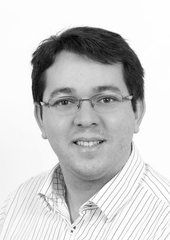
\includegraphics[width=1in,height=1.25in,clip,keepaspectratio]{lucas3por4}}]{Lucas Cordeiro}
%received his Ph.D. degree in Computer Science in 2011 from the University of Southampton, UK. Currently, he is a Senior Lecturer in the School of Computer Science at the University of Manchester, and leads the Systems and Software Verification laboratory. He is also a collaborator in the Postgraduate Program in Electrical Engineering and Informatics at the Federal University of Amazonas (UFAM), Brazil. Before joining the University of Manchester, he worked as a researcher at Oxford University / Diffblue and as an adjunct professor at UFAM; he also worked for four years as a software engineer in industry. His work focuses on software model checking, automated testing, program synthesis, and embedded \& cyber-physical systems.
%\end{IEEEbiography}
%%%%%%%%%%%%%%%%%%%%%%%%%%%%%%%%%%%%%%%%%%%%%%%%%%%%%%%%%%%%%%%%%%%%%%%%%%%%%%%%%%%
%%%%%%%%%%%%%%%%%%%%%%%%%%%%%%%%%%%%%%%%%%%%%%%%%%%%%%%%%%%%%%%%%%%%%%%%%%%%%%%%%%%
% You can push biographies down or up by placing
% a \vfill before or after them. The appropriate
% use of \vfill depends on what kind of text is
% on the last page and whether or not the columns
% are being equalized.
%\vfill
% Can be used to pull up biographies so that the bottom of the last one
% is flush with the other column.
%\enlargethispage{-5in}
% that's all folks
\end{document}